\documentclass{standalone}
\usepackage{amsmath}
\usepackage[dvipsnames]{xcolor}
\usepackage{tikz} 
\usetikzlibrary{arrows, decorations.markings,decorations.pathreplacing,angles,quotes}
\usepackage{microtype}
\usepackage{fourier}

\definecolor{nblue}{RGB}{31, 119, 180}

\begin{document}

\begin{tikzpicture}
	\node[anchor=south west,inner sep=0] (Bild) at (0,0) {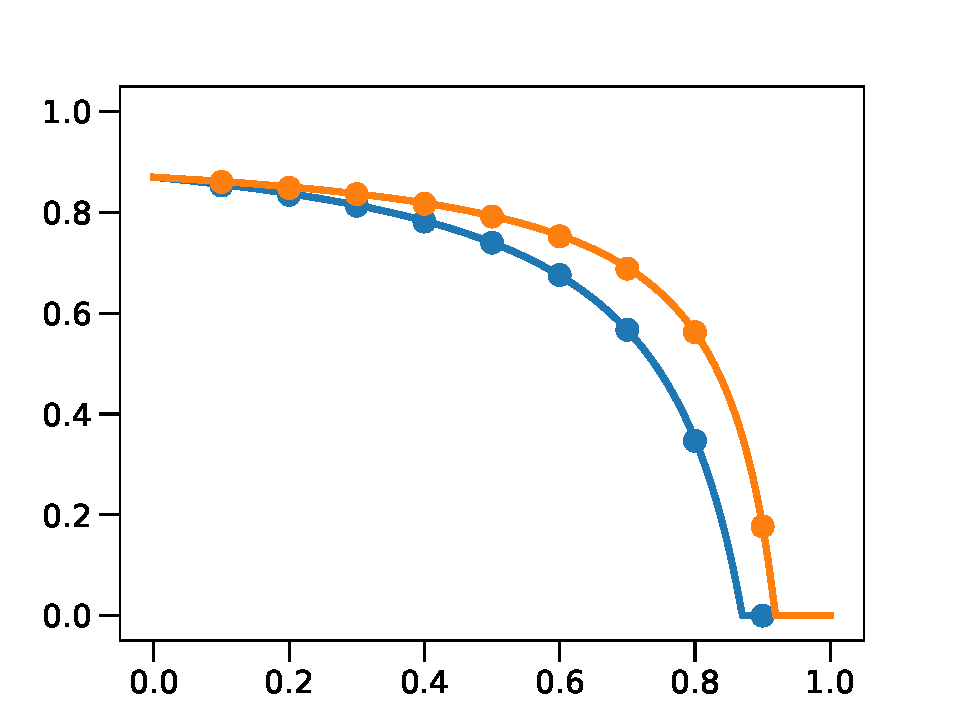
\includegraphics[scale=0.39]{figS2a_blank.pdf}};
   		\begin{scope}[x=(Bild.south east),y=(Bild.north west)]
        	\draw (0.5,-0.035) node {antiviral drug efficacy $\varepsilon_j$};
        	\draw (0.01,0.5) node [rotate=90] {establishment probability $\varphi_j$};
        	\draw[thick] (0.175,0.805) --  (0.225,0.805);
        	\draw (0.175,0.83) node[right=10pt] {\scriptsize reducing $p$,};
        	\draw (0.175,0.78) node[right=10pt] {\scriptsize increasing $\delta$};
        	\draw[thick,dashed] (0.175,0.71) -- node[right=6pt] {\scriptsize reducing $p$ and $\beta$} (0.225,0.71);
        	\draw[black,thick,dotted] (0.175,0.615) -- (0.225,0.615);
        	\draw (0.175,0.64) node[right=10pt] {\scriptsize reducing $\beta$,};
        	\draw (0.175,0.59) node[right=10pt] {\scriptsize increasing $c$};

			\draw[nblue,thick] (0.6,0.83) -- node[right=6pt] {\scriptsize \color{black} reducing $p$} (0.65,0.83);
			\draw[orange,thick] (0.6,0.78) -- node[right=6pt] {\scriptsize \color{black} reducing $\beta$}(0.65,0.78);
			
    	\end{scope}
\end{tikzpicture}

\end{document}